\documentclass[12pt]{article}

% Packages
\usepackage{amsmath, amssymb} % math symbols
\usepackage{enumitem}         % better control over lists
\usepackage{hyperref}         % clickable links
\usepackage{graphicx}

% Title Info
\title{ESE5320 Homework 1}
\author{Zhengyang "Rico" Zhuang}
\date{September 5, 2025}

\begin{document}

\maketitle

\section*{Answers}

\begin{enumerate}
    \item \textbf{GDB Tutorial}
    \begin{enumerate}[label=\arabic*)]
        \item To add a breakpoint, use \texttt{break <FUNCTION/LINE NUMBER>}.
        
        \item To delete a breakpoint, first do \texttt{"info breakpoint"} to find breakpoint index, then \texttt{"delete <INDEX>"}.
        \item To To inspect a variable's value, use \texttt{"print <VAR\_NAME>"}.
        
        \item To step through execution without a breakpoint: \texttt{next} or \texttt{step}

    \end{enumerate}

    \item  \textbf{C}
    \begin{enumerate}[label=\arabic*)]
        \item \begin{verbatim}
#include <stdio.h>
#include <stdlib.h>
#include <stdint.h>

int main(void) {
    int top = 20;
    int *p_top = &top;
    int *h50 = malloc(sizeof *h50); *h50 = 50;
    int *h5  = malloc(sizeof *h5 ); *h5  = 5;
    int *h6  = malloc(sizeof *h6 ); *h6  = 6;
    int *h7  = malloc(sizeof *h7 ); *h7  = 7;

    int *p_h50 = h50;
    int *p_h5  = h5;

    printf("Stack:\n");
    printf("%11p  %14d\n", (void*)&top, top);
    printf("%11p  %14p\n", (void*)&p_top, (void*)p_top);
    printf("%11p  %14p\n", (void*)&p_h50, (void*)p_h50);
    printf("%11p  %14p\n", (void*)&p_h5,  (void*)p_h5);

    printf("\nHeap:\n");
    printf("h50: %p = %d\n", (void*)h50, *h50);
    printf(" h5: %p = %d\n", (void*)h5,  *h5 );
    printf(" h6: %p = %d\n", (void*)h6,  *h6 );
    printf(" h7: %p = %d\n", (void*)h7,  *h7 );

    free(h50); free(h5); free(h6); free(h7);
    return 0;
}
\end{verbatim}
\begin{figure}[h]
    \centering
    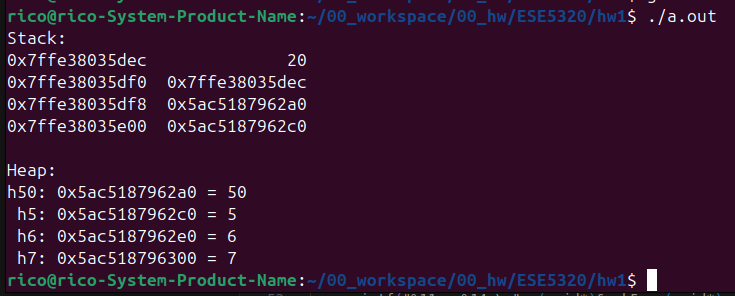
\includegraphics[width=0.7\textwidth]{image.png}
    \caption{Output from C code above}
\end{figure}

        \item \begin{verbatim}
#include <stdio.h>
int main(void) {
    int a[2][4] = { {10, 20, 30, 40}, {50, 60, 70, 80} };
    int *row[2] = { a[0], a[1] };
    for (int i = 0; i < 2; ++i) {
        for (int j = 0; j < 4; ++j) {
            printf("row[%d][%d] = %d\n", i, j, row[i][j]);
        }
    }
    return 0;
}


\end{verbatim}
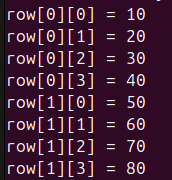
\includegraphics[width=0.3\textwidth]{image2.png}

\begin{verbatim}
#include <stdio.h>

int main(void) {
    int a[2][4] = { {10, 20, 30, 40}, {50, 60, 70, 80} };
    int *row0 = a[0];
    int *row1 = a[1];
    int *rows[2] = { row0, row1 };
    int **pp = rows;
    for (int i = 0; i < 2; ++i) {
        for (int j = 0; j < 4; ++j) {
            printf("pp[%d][%d] = %d\n", i, j, pp[i][j]);
        }
    }
    return 0;
}
\end{verbatim}
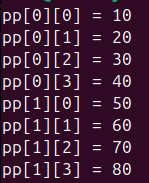
\includegraphics[width=0.2\textwidth]{image3.png}

        \item \texttt{\&x[2].d[0]->b}
        \item \begin{verbatim}
#include <stdio.h>

int main(void) {
    int a[2][4] = { {10, 20, 30, 40}, {50, 60, 70, 80} };
    int *row0 = a[0];
    int *row1 = a[1];
    int *rows[2] = { row0, row1 };
    int **pp = rows;
    for (int i = 0; i < 2; ++i) {
        for (int j = 0; j < 4; ++j) {
            printf("pp[%d][%d] = %d\n", i, j, pp[i][j]);
        }
    }
    return 0;
}
\end{verbatim}
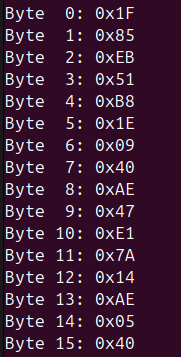
\includegraphics[width=0.3\textwidth]{image4.png}
        \item \begin{verbatim}
#include <stdio.h>
#include <stdlib.h>

void temp(int i) {
    int a[2];
    int b[3];
    int *c;
    int *d;

    c = (int *)malloc(sizeof(int) * 4);
    d = (int *)malloc(sizeof(int) * 5);

    printf("a (stack, 2 ints) : %p\n", (void*)a);
    printf("b (stack, 3 ints) : %p\n", (void*)b);
    printf("c (heap, 4 ints)  : %p\n", (void*)c);
    printf("d (heap, 5 ints)  : %p\n", (void*)d);

    free(c);
    free(d);

    return;
}

int main(void) {
    temp(0);
    return 0;
}

        \end{verbatim}
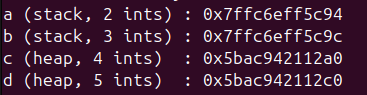
\includegraphics[width=0.6\textwidth]{image5.png}

        \item c[0] becomes 13 \\
        invaild array indexing is detected and the program stops

        \item char and unsigned char sums differ because unsigned char use all 8 bits for numbers but signed char has to use a bit for the sign, so they overflow at different sums
        \\\\char and unsigned char sums differ from their 'intsum' because intsum can use 32bits but chars can only use 8 so they overflow after 255.

        \item Preprocessor: Handles stuff like include and define before compiling 
        \\compiler: Translates the preprocessed C code into assembly or machine code 
        \\Linker: Combines object files and libraries into executable

        \item add the include path to the makefile -I \\ copy the headerfile to local directory \\ check name and path to make sure that they are correct
        \item object file missing \\ function not defined \\ function signature does not match
    \end{enumerate}

    \item \textbf{Debug an Application}
    \begin{enumerate}[label=\arabic*)]
        \item Done
        \item Done
        \item Done
        \item \begin{enumerate}[label=\arabic*)]
        \item On line 5 I changed \texttt{"while (*s) s++;"} to \texttt{"while (*s++) l++;"}
        \item Makefile: \begin{verbatim}
release:
	gcc -Wall -o program program.c

debug:
	gcc -g -Wall -o program program.c
        \end{verbatim}
        \item The secret message is: Well Done!!
        \item while loop not executed at all, must be buggy len(). Steppting through len, l doesn't change at all. Look back at the code and noticed that s is incremented  in while loop but l is not. 
        \end{enumerate}
        \item the -g flag of gcc adds debug symbols that maps addresses back to source files, and is read by gdb

    \end{enumerate}

\end{enumerate}

\end{document}
